% $Id$
% Author:	Daniel Bosk <daniel.bosk@miun.se>
%\documentclass[handout]{beamer}
\documentclass{beamer}
\usepackage[utf8]{inputenc}
\usepackage[T1]{fontenc}
\usepackage[swedish,english]{babel}
\usepackage[babel=true]{csquotes}
\usepackage{url}
\usepackage{graphicx}
\usepackage[today,nofancy]{svninfo}
\usepackage[natbib,style=alphabetic,maxbibnames=99,backend=bibtex8]{biblatex}
\addbibresource{literature.bib}

\svnInfo $Id$

\mode<presentation>
{
  \usetheme{Frankfurt}
  \setbeamercovered{transparent}
  \usecolortheme{seagull}
}
\setbeamertemplate{footline}{\insertframenumber}

\title{%
  Introduction to \\
  Operating Systems
}
\author{Daniel Bosk\footnote{%
	\tiny
  This work is licensed under the Creative Commons Attribution-ShareAlike 3.0 
  Unported license.
	To view a copy of this license, visit 
	\url{http://creativecommons.org/licenses/by-sa/3.0/}.
}}
\institute[MIUN ICS]{%
  Department of Information and Communication Systems (ICS),\\
  Mid Sweden University, Sundsvall.
}
\date{\svnId}


\AtBeginSection[]{%
	\begin{frame}<beamer>{Overview}
		\tableofcontents[currentsection]
	\end{frame}
}

\begin{document}

\begin{frame}
  \titlepage
\end{frame}

\begin{frame}{Overview}
	\tableofcontents
	% You might wish to add the option [pausesections]
\end{frame}


% Since this a solution template for a generic talk, very little can
% be said about how it should be structured. However, the talk length
% of between 15min and 45min and the theme suggest that you stick to
% the following rules:  

% - Exactly two or three sections (other than the summary).
% - At *most* three subsections per section.
% - Talk about 30s to 2min per frame. So there should be between about
%   15 and 30 frames, all told.


\section{Formalia}

\subsection{Schedule}

\begin{frame}{\insertsubsectionhead}
  \begin{itemize}
    \item The schedule is in the central scheduling system in the Student 
      Portal.

    \item This schedule is not synchronised with that in the virtual learning 
      environment (Moodle).

    \item The sessions and lectures in the schedule are the only ones offered, 
      so there are no sessions planned after the course.

  \end{itemize}
\end{frame}

\subsection{Literature}

\begin{frame}{\insertsubsectionhead}
  \begin{itemize}
%    \item \citetitle{Silberschatz2009osc}, 8th edition 
%      \cite{Silberschatz2009osc}.

    \item \citetitle{Silberschatz2013osc}, 9th edition 
      \cite{Silberschatz2013osc}.

  \end{itemize}
\end{frame}

\subsection{Virtual Learning Environment}

\begin{frame}{\insertsubsectionhead}
  \begin{itemize}
    \item The virtual learning environment (VLE) used for the course is 
      ''Lärplattformen 2.0'', i.e.\ Moodle.

    \item In the section ''Course Material'' found in the VLE you will find 
      recordings of lectures and lecture slides.

    \item In the section ''Examination'' you will find all things related to 
      the examination, i.e.\ hand-in assignments.

    \item In each hand-in box you will find the instruction for that particular 
      assignment.

    \item Read the instructions carefully!

    \item The hand-in assignments are numbered starting on 0 and are prefixed 
      with a letter indicating the type of assignment.
      Theory assignments are prefixed T and laboratory assignments are prefixed 
      L.

  \end{itemize}
\end{frame}

\subsection{Examination}

\begin{frame}{\insertsubsectionhead}
  \begin{itemize}
    \item The first theory assignment, T0, is mandatory.

    \item The other assignments are not mandatory, but they will give bonus 
      points if completed on time.

    \item Final exam the last week of the course.

  \end{itemize}
\end{frame}

\begin{frame}{\insertsubsectionhead}{Hand-ins}
  \begin{itemize}
    \item T0 Overview
    \item T1 Processes
    \item T2 Memory
    \item L3 Paging Algorithms
    \item T4 Storage
%    \item T5 Distributed Systems
  \end{itemize}
\end{frame}

\begin{frame}{\insertsubsectionhead}{Final exam}
  \begin{itemize}
    \item The final exam will cover the entire course.
    \item The hand-in assignments serve as a good preparation for the exam.
  \end{itemize}
\end{frame}


\section[History]{The History of UNIX}

\subsection[Development]{The development of UNIX}

\begin{frame}{\insertsubsectionhead}
  \begin{itemize}
    \item UNIX was originally developed at Bell Labs.
    \item This timeline is derived from documents in Bell Labs' historical 
      archive \cite{BellLabs2002tco}.
  \end{itemize}
\end{frame}

\begin{frame}{Development timeline}{The 1960s}
	\begin{description}
		\item<1>[1965]
			Multiplexed Infomation and Computing Service (MULTICS) was a joint effort 
			between MIT, Bell Labs and GE to

			\begin{quote}
        ``develop a convenient, interactive, useable computer system that could 
        support many users'' \cite{BellLabs2002tco}.
			\end{quote}

		\item<2>[1969]
			\begin{itemize}
				\item Bell Labs withdrew from the project, but Ken Thompson, Dennis 
					Ritchie, Douglas McIllroy, and J. F. Ossanna continued on their own.

				\item	Started to write the system on a PDP-7, at first simply as a file 
					system.

				\item The system then got a shell, an editor, and an assembler.

			\end{itemize}

	\end{description}
\end{frame}

\begin{frame}{Development timeline}{The 1970s}
	\begin{description}
		\item<1>[1970]
			\begin{itemize}
				\item Brian Kernighan suggests the name UNIX.

				\item They port the current code to a PDP-11.

				\item Focused for use in text-processing, patent applications for 
					Bell Labs.

			\end{itemize}

		\item<2->[1971] Ritchie improved Thompson's B programming language into the 
			C programming language.

		\item<3>[1972] Thompson started rewriting UNIX in C.
			(And continuous improvement of C.)

	\end{description}
\end{frame}

\begin{frame}{Development timeline}{The 1970s, continued}
	\begin{description}
		\uncover<1>{
		\item[1973]
			\begin{itemize}
				\item UNIX completely rewritten in C.
				\item Thompson added McIlroy's concept of pipes.
					With this came the UNIX philosophy:
			\end{itemize}
		}
		\uncover<2>{
			\begin{quote}
				``Write programs that do one thing and do it well.
				Write programs to work together.
				Write programs that handle text streams, because that is 
				a universal interface.'' \cite{BellLabs2002tco}
			\end{quote}
		}
		\uncover<3>{
			\begin{itemize}
				\item Ritchie took initiative to manual pages, McIlroy soon took over 
					and is the mind behind the layout of manual pages.
      \end{itemize}
		}
	\end{description}
\end{frame}

\begin{frame}{Development timeline}{The 1970s, continued}
	\begin{description}
		\item<1>[1975] Thompson is visiting professor at University of 
			California-Berkeley (UCB).
			While there he developed version 6 of UNIX.

		\item<2>[1978] Professors at Berkeley continued the enhancement of UNIX and 
			distributed their work as Berkeley Software Distribution (BSD).

  \end{description}
\end{frame}

\begin{frame}{Development timeline}{The 1980s}
	\begin{description}
		\item<1>[1983]
			\begin{itemize}
				\item Sockets API added to BSD (4.2BSD), i.e. TCP/IP made easily 
					available.

				\item David Korn develops the Korn Shell scripting language.

				\item Bjarne Stroustrup develops the first version of C++.

			\end{itemize}

		\item<2>[1984] AT\&T, owner of Bell Labs, started selling UNIX-licenses to 
			companies.

  \end{description}
\end{frame}

\begin{frame}{Development timeline}{Present}
	To this day, UNIX-like operating systems operate ``most large Internet 
	servers, businesses and universities, and a major part of academic and 
	industrial research in operating systems is based on UNIX'' 
	\cite{BellLabs2002tco}.
\end{frame}

\subsection{Evolution of UNIX}

\begin{frame}{\insertsubsectionhead}
  \begin{figure}
    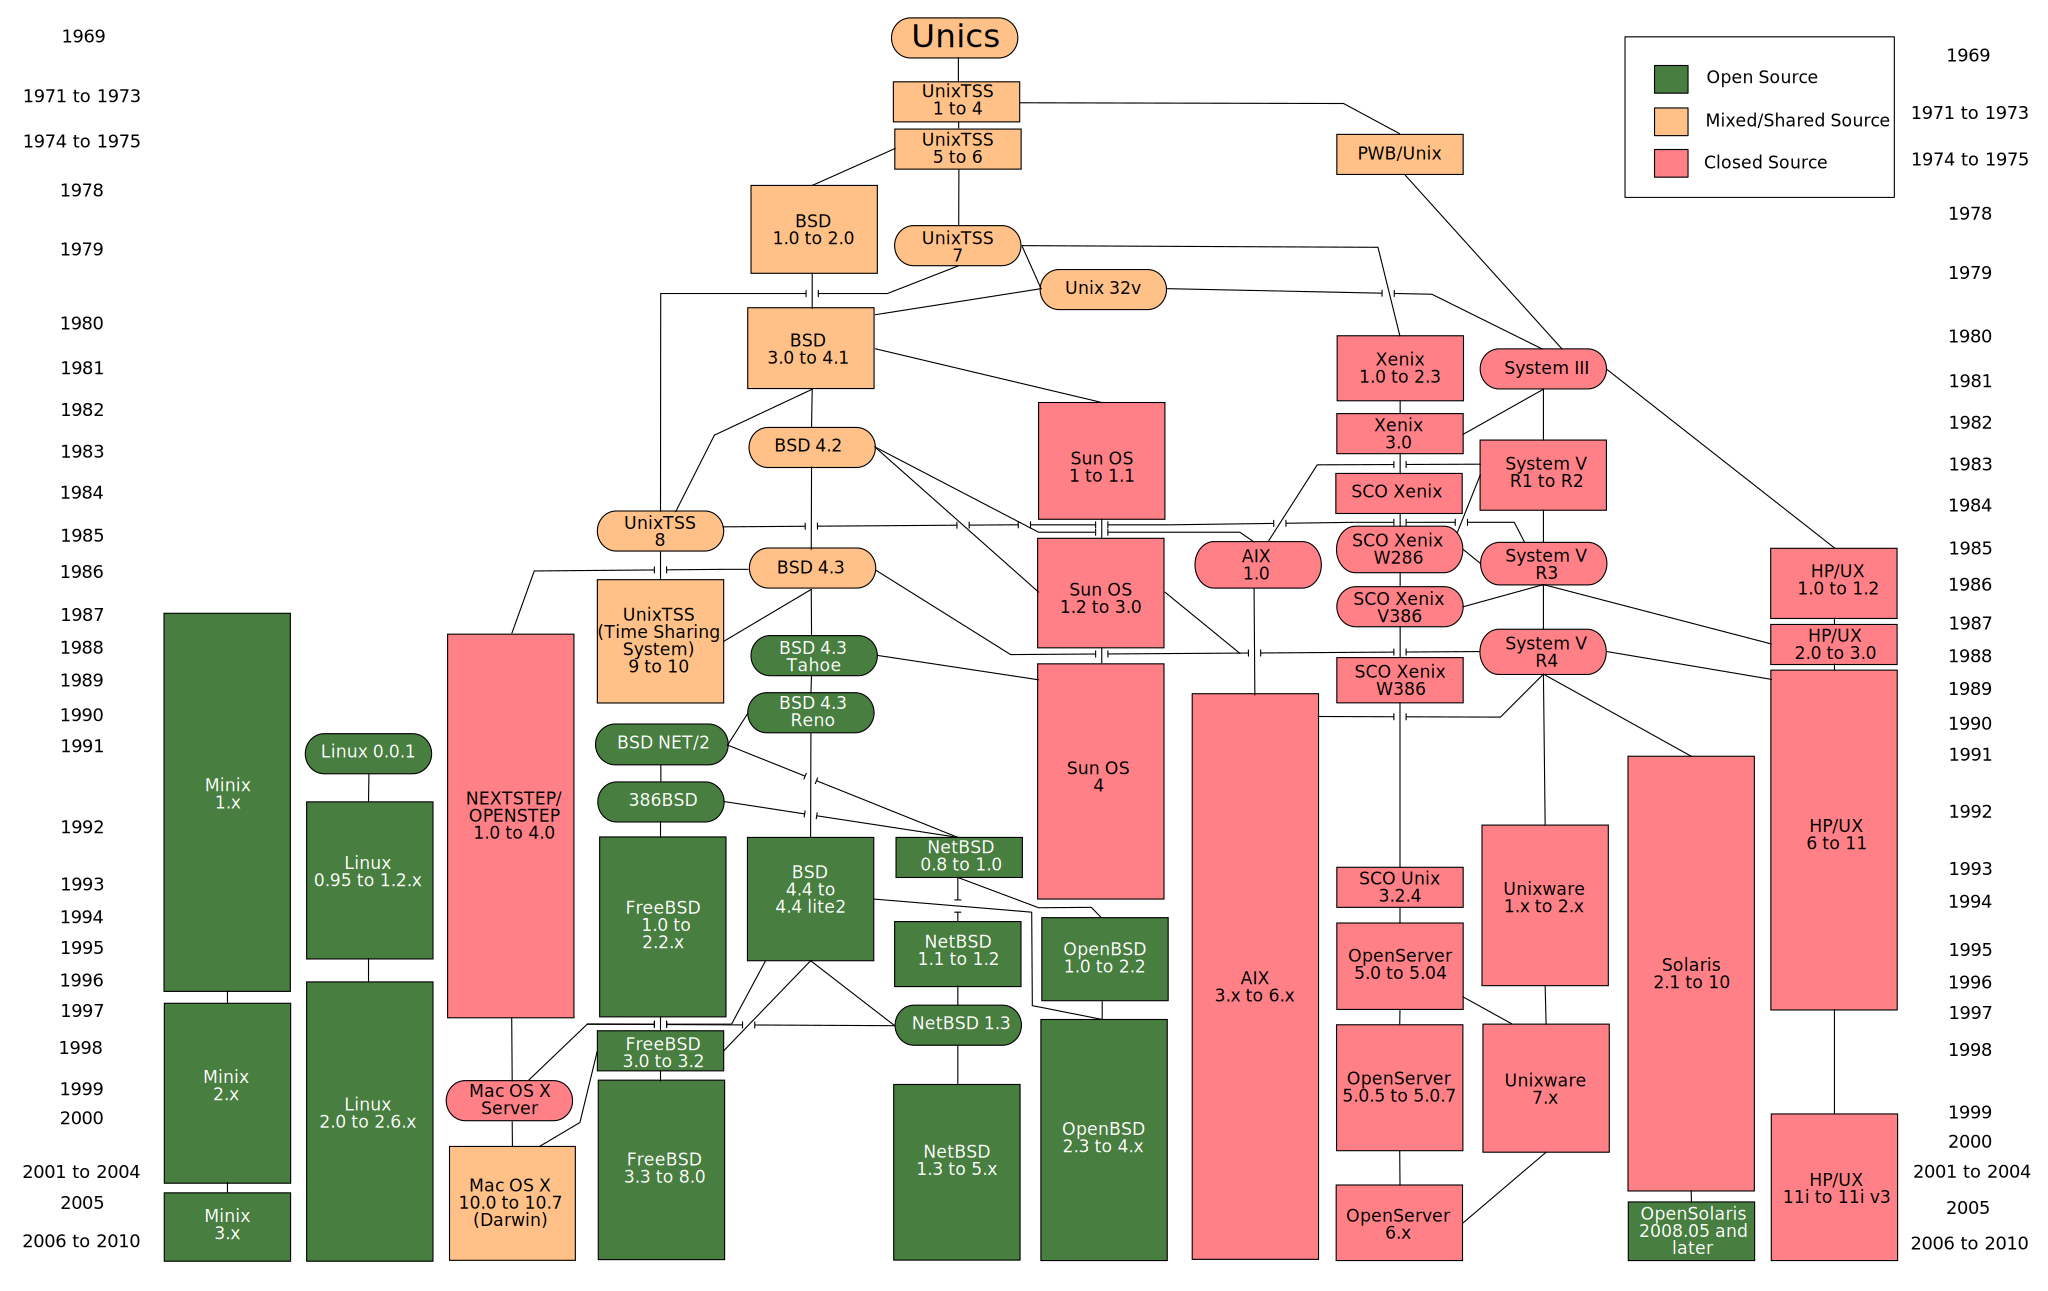
\includegraphics[width=\textheight]{Unix_history-simple.pdf}
    \caption{A simplified overview of UNIX history.
    For details see \url{http://www.levenez.com/unix/}.
    Image: \url{https://en.wikipedia.org/wiki/File:Unix_history-simple.svg}.
  }
  \end{figure}
\end{frame}


%%%%%%%%%%%%%%%%%%%%%%

\begin{frame}[allowframebreaks]{Referenser}
  \small
  \printbibliography
\end{frame}

\end{document}

